
\section{Durchführung}
\label{sec:Durchführung}
\renewcommand{\labelenumi}{\alph{enumi})}
\begin{enumerate}


  \begin{figure}[H]
    \centering
    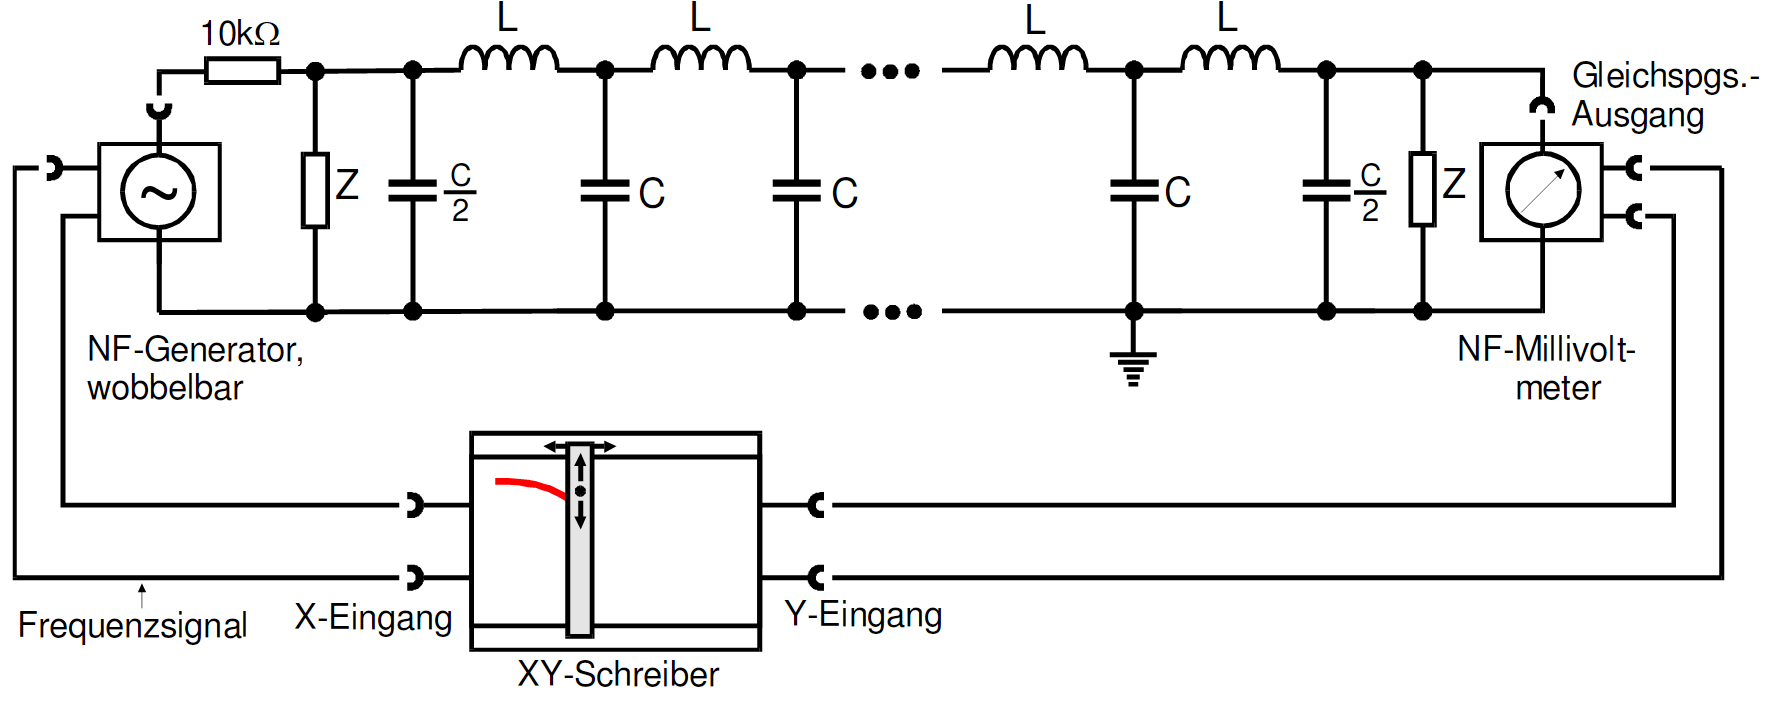
\includegraphics[width=\linewidth-120pt,height=\textheight-120pt,keepaspectratio]{content/Grafiken/Schaltunga.png}
    \caption{Schaltung zum Aufzeichnen der Durchlasskurven \cite{V356}.}
    \label{fig:Schaltung1}
  \end{figure}

  \item Zunächst werden Durchlasskurven der $LC$ und $LC_1C_2$-Kette aufgenommen.
   Hierzu wird die jeweilige Kettenschaltung gemäß Abb. 3 an einen XY-Schreiber
   angeschlossen. Um das Verhalten einer unendlichen Kette zu erzeugen, werden die
   variablen Widerstände an den Enden der Kette auf den nach (1) berechenbaren
   Wellenwiderstand eingestellt. Am Generator wird eine Sinusspannung gewählt.
    Aufgrund von älteren Geräten wird die Wechselspannungsfrequenz über einen
     Frequenzmesser abgelesen. Auch beide Abschlusswiderstände werden mithilfe
      eines Ohmmeters justiert. Während des Schreibvorganges sind die Frequenzen
       an verschiedenen Stellen der X-Achse zu notieren, um eine Skala dieser zu erhalten.
        Es ist zu beachten, dass die X-Achse der
       Graphen $\propto \ln(f)$ verläuft.

       \begin{figure}[H]
         \centering
         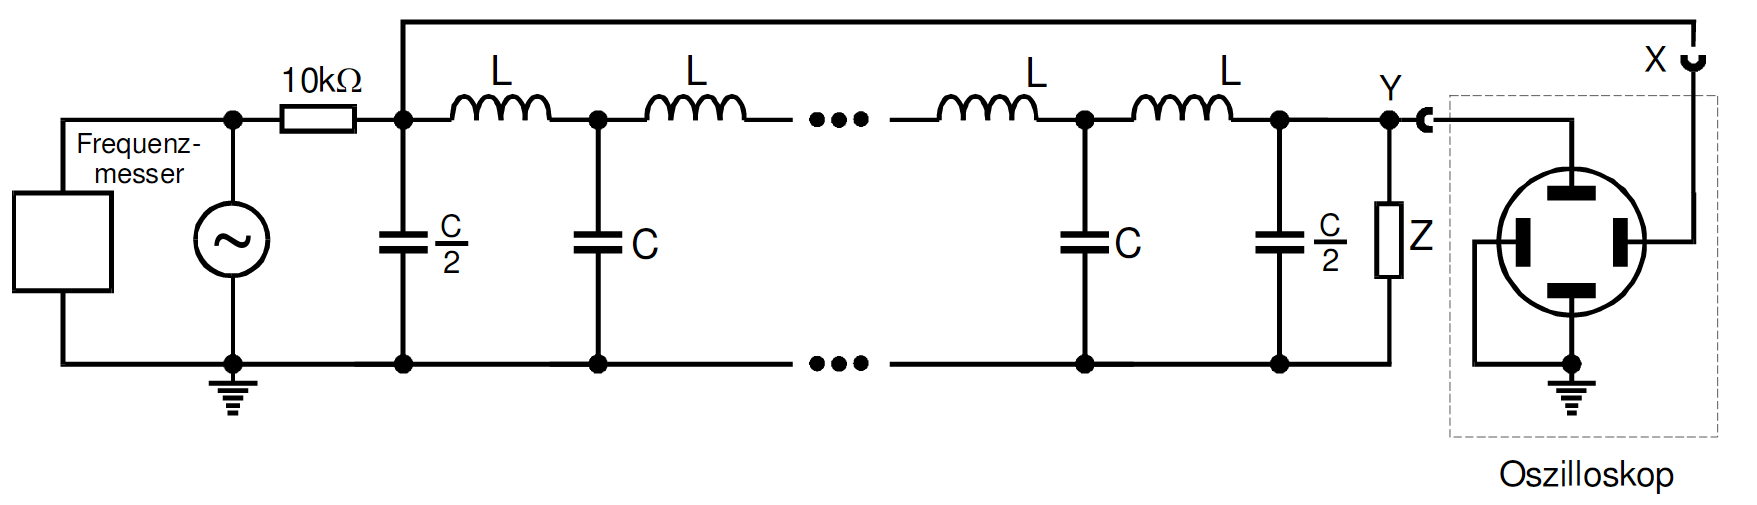
\includegraphics[width=\linewidth-120pt,height=\textheight-120pt,keepaspectratio]{content/Grafiken/Schaltungb.png}
         \caption{Messschaltung zum aufnehmen des Dispersionsverhaltens \cite{V356}.}
         \label{fig:Schaltung2}
       \end{figure}

\item Als nächstes wird die Dispersionsrelation überprüft. Hierzu wird die
 Kettenschaltung gemäß Abb. 4 integriert. Das Oszilloskop
  wird auf den XY-Modus eingestellt. Anschließend werden alle Frequenzen notiert,
    bei denen die auftretende Lissajous-Figur die Form einer Gerade hat. Dies ist der
     Fall, wenn die gesamte Phasenänderung auf der Kettenschaltungen ein
      Vielfaches von $\pi$ erreicht. Die gesuchte Phasenverschiebung pro Kettenglied
       wird erreicht, indem man durch die Anzahl der Kettenglieder teilt.

\item Es wird nun auf eine beiderseits offene $LC$-Kette gewechselt. Hierzu kann
 die bereits aus Durchführungsteil a) bekannte Schaltung verwendet werden,
  jedoch ohne Schreiber und Wobbeleinrichtung. Um zwei offene Enden zu
   erzeugen, werden beide Abschlusswiderstände entfernt und der Stromkreis geöffnet.
    Auf der LC-Kette bilden sich nun stehende Wellen.
   Es werden die Frequenzen notiert, bei denen die Spannung am Kettenende
    maximal ist. Hierzu wird ein Millivoltmeter zwischengeschaltet.

\item Anschließend werden zu den ersten beiden Eigenschwingungen auch die
 jeweiligen, an den einzelnen $LC$-Gliedern anliegenden, Spannungen notiert. Hierzu wird
  das ausgehende Kabel nicht mehr am Kettenschaltungsende angebracht, sondern
   am jeweiligen $LC$-Glied.

   \item Zuletzt wird die letzte Messung nochmals durchgeführt, diesmal
   haben die Abschlusswiderstände jedoch den Wert des Wellenwiderstandes.
    Der Stromkreis wird daher wieder geschlossen.
     %die Abschlusswiderstände werden
     %wieder eingesetzt und nochmals justiert.


\end{enumerate}
